\documentclass[11pt, oneside]{article} 
\usepackage{geometry}
\geometry{letterpaper} 
\usepackage{graphicx}
	
\usepackage{amssymb}
\usepackage{amsmath}
\usepackage{parskip}
\usepackage{color}
\usepackage{hyperref}

\graphicspath{{/Users/telliott_admin/Tex/png/}}
% \begin{center} 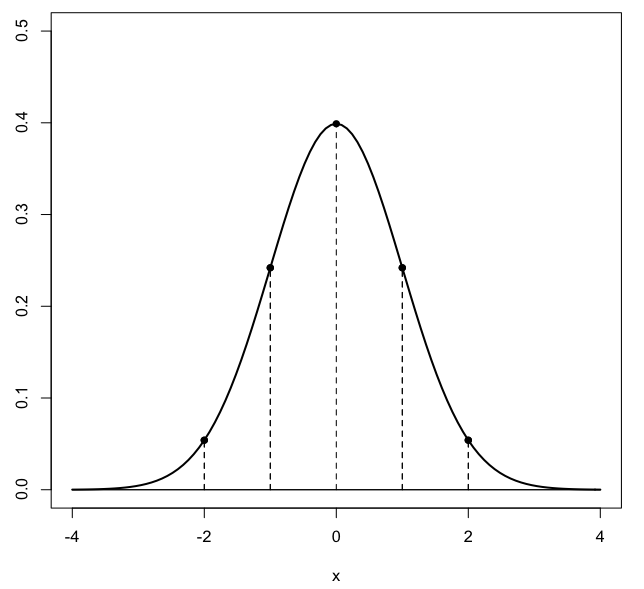
\includegraphics [scale=0.4] {gauss3.png} \end{center}

%break
\title{Exponential and Logarithm}
\date{}

\begin{document}
\maketitle
\Large

\subsection*{The exponential is its own derivative}

As we've emphasized, the most important fact about the exponential function $f(x) = e^x$ is that this function is its own derivative.  

Above, we derived the famous series for
\[ e^x = \sum_{n=0}^{\infty} \frac{x^n}{n!} = \frac{x^{0}}{0!} + \frac{x^{1}}{1!} + \frac{x^{2}}{2!} + \cdots  \]

Note that a good approximation for small $x$ is
\[ e^x \approx 1 + x \]

If you need more precision, you can add another term:
\[ e^x \approx 1 + x + \frac{x^2}{2!} \]


It is easy to see that the derivative of this series is the series itself.

Take $\frac{d}{dx}$ of the last series.

\[ \frac{d}{dx} \ e^x = 0 + (1)\frac{x^{1-1}}{1!} + (2)\frac{x^{2-1}}{2!} + (3)\frac{x^{3-1}}{3!} + \cdots  \]
\[ \frac{d}{dx} \ e^x = 0 + \frac{x^{0}}{0!} + \frac{x^{1}}{1!} + \frac{x^{2}}{2!} + \cdots  \]
\[ = e^x \]
Each exponent $n$ that comes down through the power rule, finds an $n$ in $n!=n \times (n-1) \times (n-2) \dots $ to cancel, leaving $n-1$ in the exponent as well as $(n-1)!$.

\subsection*{from exponential to logarithm}
It is possible to obtain the definition of the derivative of the logarithm from the definition:
\[ \int \frac{1}{t} \ dt = \ln(t) \]
Differentiate both sides.  By the FTC:
\[ \frac{d}{dt} \int \frac{1}{t} \ dt  = \frac{1}{t}  = \frac{d}{dt} \ln(t) \]
This is great because we never did generate $x^{-1}$ by differentiating powers of $x$.  

Now we know how to go back the other way, using the definition that the exponential function is its own derivative to establish the first statement above.

The proof is so simple that if you blink, you'll miss it.
\[ y = e^x \]
\[ \frac{d}{dx} e^x = \frac{dy}{dx} = e^x  \]
\[ \frac{dy}{dx} = y \]
Invert
\[ \frac{dx}{dy} = \frac{1}{y} \]
\[ dx = \frac{1}{y} \ dy \]
Integrate
\[ \int dx = x = \int \frac{1}{y} \ dy \]
And what is $x$?  It is $\ln y$!
\[ \ln(y) = \int \frac{1}{y} \ dy \]
And since $y$ is just a letter, we can write the same for $x$, or $t$
\[ \ln x = \int \frac{1}{x} \ dx \]
\[ \ln t = \int \frac{1}{t} \ dt \]
One of the prettiest things I've ever seen.

The math purists don't like it, but in general it is OK to do algebra with differentials.  One important restriction is that $dy/dx$ (and $dx/dy$) should not be equal to zero.  And a second one is that we just remember we are never passing to the limit, just getting really, really, really close.  (As close as you like).

Now that we have this definition, we have another way of estimating the value of $e$.  We add up the areas for little slices under the function $y=1/x$ until the total reaches $1$.  The corresponding value of $x=e$.
\begin{center}
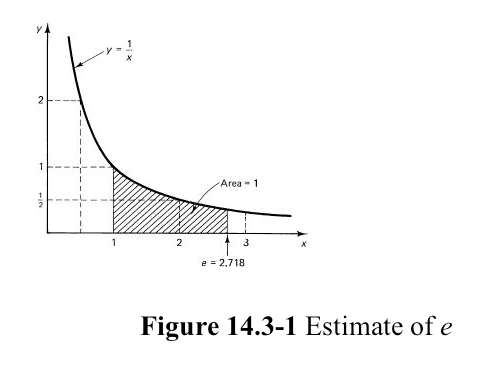
\includegraphics [scale=0.6] {log3.png}
\end{center}
(from Hamming's \emph{Calculus}).

For example, we might try intervals of $0.1$ and do
\[ 0.1 \cdot \frac{1}{1} + 0.1 \cdot \frac{1}{1.1} + 0.1 \cdot \frac{1}{1.2} + \dots + 0.1 \cdot \frac{1}{2.7} \]

\subsection*{reverse direction}
From above, we had
\[ \ln x = \int \frac{1}{x} \ dx \]
Differentiate both sides
\[ {\frac{d}{dx} \ln(x) = \frac{1}{x} } \]
We want to go backward now, to show that the derivative of the function $f(x) = e^x$ is itself.

Start with
\[ \ln(e^x) = x \]
\[ \frac{d}{dx} \ln(e^x) = \frac{d}{dx} x = 1 \]
but using the property we just proved and the chain rule, this is also
\[ \frac{d}{dx} \ln(e^x) = \frac{1}{e^x} \ \frac{d}{dx} e^x  \]
so these two expressions are equal and
\[ \frac{1}{e^x} \ \frac{d}{dx} e^x = 1  \] 
\[ \frac{d}{dx} e^x = e^x \]

Magic.

\subsection*{Strang's view of the series}

Gil Strang has a nice introduction to the exponential (for real numbers).  He says we want to "construct a function" for $y = e^x$.  The first, amazing, property ($I$) that it has is that the derivative of the function is equal to the function itself.
\[ \frac{dy}{dx} = y \]
This is our first differential equation.

The second property, a boundary condition, is that at $x = 0$, we want $y = 1$.  That's because $e$ is not a variable and we want $e^x = e^0$ to be equal to $1$ like every other exponential we know.  [ A third property that will turn out to be true is $e^{x_1 + x_2} = e^{x_1} \cdot e^{x_2}$. ]

Using the second condition we write:
\[ y(x) = 1 \]
Whatever else is true, if there are no terms containing $x$ (because $x=0$) then $y = 1$.  By $I$ we must have that the derivative is equal to the function:
\[ y(x) = 1 \]
\[ \frac{dy}{dx} = 1 \]
But now, if we try to evaluate the derivative starting from $y(x)$, where does that $1$ come from?  It must come from
\[ y(x) = 1 + x \]
\[ \frac{dy}{dx} = 1 \]
Now, though, it's no longer true that $y = dy/dx$ so we fix that
\[ y(x) = 1 + x \]
\[ \frac{dy}{dx} = 1 + x \]
And where does that $x$ come from in the derivative?  It must come from
\[ y(x) = 1 + x + \frac{x^2}{2} \]
\[ \frac{dy}{dx} = 1 + x \]
And so on ...  Following this procedure, we build up the definition
\[ y(x) = \sum_0^{\infty} \frac{x^n}{n!} \]

The test for convergence is to find $x$ such that:
\[ \lim_{n \rightarrow \infty} \frac{|A_{n+1}|}{|A_n|} < 1 \]
\[ = \lim_{n \rightarrow \infty} \frac{x}{n+1} \]
But this is true for any $x$.


\end{document}